\chapter{Descripción del Trabajo Realidad Aumentada}
\label{cap:descripcionTrabajo}

%  Aquí comienza la descripción del trabajo realizado. Se deben incluir tantos capítulos como sea necesario para describir de la manera más completa posible el trabajo que se ha llevado a cabo. Como muestra la figura \ref{fig:sampleImage}, está todo por hacer.

% \begin{figure}[h]
% 	\centering
% 	
\includegraphics[width = 0.5\textwidth]{Imagenes/Vectorial/Todo.pdf}
% 	\caption{Ejemplo de imagen}
% 	\label{fig:sampleImage}
% \end{figure}

% Si te sirve de utilidad,  puedes incluir tablas para mostrar resultados, tal como se ve en la tabla \ref{tab:sampleTable}.


% \begin{table}
% 	\centering
% 	\begin{tabular}{c|c|c}
% 		\textbf{Col 1} & \textbf{Col 2} & \textbf{Col 3} \\
% 		\hline\hline
% 		3 & 3.01 & 3.50\\
% 		6 & 2.12 & 4.40\\
% 		1 & 3.79 & 5.00\\
% 		2 & 4.88 & 5.30\\
% 		4 & 3.50 & 2.90\\
% 		5 & 7.40 & 4.70\\
% 		\hline
% 	\end{tabular}
% 	\caption{Tabla de ejemplo}
% 	\label{tab:sampleTable}
% \end{table}
\chapterquote{En Chiloeches la prisa se disuelve en el color de sus tierras y el eco de su historia}{Antonio Herrera Casado}
El trabajo descrito en este capítulo es un plugin para \textit{OBS Studio} que convierte cualquier retransmisión de vídeo en una experiencia de realidad aumentada orientada a concursos de programación. El plugin detecta marcadores \textbf{ArUco} \citep{GarridoJurado2014} impresos sobre las mesas del concurso, estima su posición y orientación exactas en el espacio real, y sobre ese anclaje físico superpone contenido virtual: modelos 3D arbitrarios, un cronómetro analógico sincronizado con el servidor del juez, y paneles de texto con la clasificación general o los datos del equipo que la cámara está captando en ese momento. Todo ello ocurre en tiempo real dentro del propio cadena de procesamiento de vídeo de \textit{OBS Studio}, sin software externo ni procesado adicional, de modo que el operador gestiona el sistema desde el mismo panel con el que controla el resto de la retransmisión.

Siguiendo la taxonomía descrita en \ref{sec:tipos_ra}, el sistema desarrollado se caracteriza, en primer lugar, por ser de tipo visión vídeo transparente. En esta modalidad, la imagen del mundo real es capturada por la cámara del equipo de retransmisión y el contenido digital se integra sobre el flujo de vídeo antes de ser visualizado por el espectador. En cuanto a la integración de elementos, se ha optado por una \textbf{RA aditiva}: esto implica que los gráficos virtuales se superponen a la escena capturada para enriquecerla, sin sustituir ni ocultar elementos físicos existentes. Esta es la aproximación más natural y efectiva en el ámbito de la retransmisión profesional, ya que permite mantener la integridad visual del evento mientras se añade información de valor.
Finalmente, como decisión de diseño central de este proyecto y con el objetivo de aprovechar las capacidades de la librería OpenCV, se ha implementado un sistema  basado en marcadores. Hemos decidido utilizar específicamente marcadores \textbf{ArUco} debido a su excelente integración con OpenCV, lo que permite un seguimiento robusto y eficiente. Estos marcadores, detallados técnicamente en la sección \ref{subsec:opencv}, facilitan la detección y el posicionamiento de los elementos digitales sobre las mesas de juego, permitiendo una implementación precisa dentro del entorno real del TFG.

El desarrollo cubre tres grandes áreas técnicas. La primera es el motor de renderizado 3D integrado en OBS, capaz de cargar modelos en múltiples formatos, aplicar cadenas de transformaciones espaciales y animar las manecillas del cronómetro fotograma a fotograma. La segunda es el sistema de visión por computador, basado en \textbf{OpenCV} y en una calibración previa de la cámara, que resuelve en tiempo real la posición y orientación de cada marcador respecto a la lente. La tercera es la capa de conectividad asíncrona que, mediante \textbf{libcurl}, mantiene sincronizados los datos del concurso con la API de \textbf{DOMjudge} sin interferir en ningún momento con el hilo de renderizado.

\section{Decisión arquitectónica: fuente o filtro}
\label{sec:decision_fuente_filtro}

Decidir integrar la RA como plugin nativo de OBS, en lugar de como aplicación externa, es solo el primer paso. Dentro del modelo de plugins de OBS Studio, descrito en la sección~\ref{sec:obs_studio}, existen dos mecanismos distintos mediante los que un plugin puede inyectar contenido en la cadena de procesamiento de vídeo, y la elección entre ambos no es trivial: condiciona qué datos recibe el plugin, qué puede hacer con ellos y cómo interactúa con el resto de la escena. Antes de abordar la implementación, conviene reconstruir el análisis que llevó a la decisión final.

\subsection{Las dos alternativas }
\label{subsec:alternativas_obs}

La primera alternativa es implementar el sistema como una \textbf{fuente de vídeo}. En este modelo, el operador añade a la escena un nuevo tipo de fuente registrado por el plugin. En cada fotograma, OBS invoca un \textit{callback} sobre esa fuente solicitándole una imagen completa. El plugin tiene libertad total para construir esa imagen como considere oportuno: puede capturar una cámara, procesar el fotograma y devolver el resultado combinado con los gráficos de RA.

La segunda alternativa es implementarlo como un \textbf{filtro de vídeo}. En este modelo, el plugin se adjunta a una fuente de cámara ya existente en la escena. En cada fotograma, OBS proporciona al filtro el fotograma que acaba de producir esa fuente y le solicita que devuelva ese mismo fotograma modificado. El plugin recibe la imagen de cámara sin tener que gestionarla, aplica la lógica de RA sobre ella y entrega el resultado.

 OBS establece que con cada tipo es, por tanto, diferente. A una fuente le pide que produzca una imagen. A un filtro le pide que transforme una imagen que ya existe. Esta distinción, que parece sutil desde el punto de vista del usuario, tiene consecuencias importantes a nivel de API.

\subsection{Análisis del API: qué puede hacer cada tipo}
\label{subsec:analisis_api}

Para tomar una decisión fundamentada fue necesario responder dos preguntas concretas consultando la API de OBS.

La primera pregunta era si, \textbf{desde una fuente}, el plugin podría acceder a la señal de vídeo de una cámara ya configurada en la escena. La respuesta que se obtuvo del análisis de la API es que OBS no proporciona un mecanismo directo para que una fuente lea los fotogramas de otra fuente activa en tiempo real. Conseguirlo requeriría duplicar la captura de la cámara dentro del plugin, con el coste de procesar dos veces la misma señal, o implementar un mecanismo de compartición de texturas entre fuentes, lo que añade complejidad, puntos de fallo y una latencia adicional de al menos un fotograma.

La segunda pregunta era si, \textbf{desde un filtro}, el plugin podría renderizar geometría 3D arbitraria sobre el fotograma recibido. La respuesta aquí fue afirmativa. El \textit{callback} de renderizado de un filtro recibe el contexto gráfico de OBS con acceso completo a la GPU: sombreadores, \textit{vertex buffers}, matrices de transformación y primitivas de dibujo. No existe ninguna restricción sobre el tipo de contenido que se puede dibujar dentro de ese contexto, únicamente sobre cuándo ocurre, dentro del ciclo de renderizado del fotograma actual.

\subsection{Decisión y consecuencias para la implementación}
\label{subsec:decision_filtro}

Con ese análisis sobre la mesa, la elección recayó sobre el \textbf{filtro de vídeo}. Resuelve favorablemente las dos preguntas del análisis anterior: el fotograma de cámara llega al plugin sin que este tenga que gestionarlo, y el renderizado 3D sobre él es plenamente posible. A ello se suman dos ventajas operativas relevantes para el uso en producción. El filtro es no destructivo: puede activarse y desactivarse en cualquier momento desde el panel de OBS sin afectar al resto de la escena ni a la configuración de la cámara. Y el operador no altera su flujo de trabajo habitual, ya que la fuente de cámara permanece intacta y el filtro se añade sobre ella desde el menú de filtros de OBS.

La consecuencia directa sobre la implementación es que el plugin registra dos \textit{callbacks} ante la API de OBS. El primero es el \textit{callback} de vídeo, que recibe cada fotograma entrante de la cámara y ejecuta sobre él la detección de marcadores ArUco. El segundo es el \textit{callback} de renderizado, que toma el resultado de esa detección y compone la geometría 3D sobre el fotograma. Ambos \textit{callbacks} se ejecutan en el hilo principal de OBS, lo que impone una restricción fundamental: ninguno de los dos puede realizar operaciones bloqueantes, como peticiones de red, sin detener la producción de fotogramas. Esta restricción es la que motiva la arquitectura de dos hilos descrita en la sección~\ref{subsec:hilos}.

\section{Ciclo de vida del plugin}
\label{sec:ciclo_vida}

El ciclo de ejecución del plugin se rige por el modelo de \textit{callbacks} de OBS Studio. OBS invoca estas funciones en el momento adecuado; el plugin solo registra qué debe hacer en cada una. El resultado es un flujo de tres fases que se repite fotograma a fotograma durante toda la retransmisión.

\subsection{Inicialización}
La fase de inicialización ocurre una única vez cuando el operador añade el filtro a una fuente de vídeo en OBS. El plugin carga los parámetros de calibración de cámara, instancia el detector ArUco con el diccionario configurado y transfiere la geometría de los modelos 3D a la memoria de la GPU.

\subsection{Actualización de lógica}
OBS invoca el \textbf{callback de vídeo} una vez por cada fotograma entrante. El plugin convierte el fotograma al formato que requiere OpenCV, ejecuta la detección de marcadores ArUco, estima la pose del marcador detectado y aplica el suavizado sobre el resultado.

\subsection{Renderizado gráfico}
El \textbf{callback de renderizado} se invoca a continuación, también en el hilo principal. A partir del estado calculado en el \textit{callback} anterior, configura el contexto gráfico de OBS, aplica la cadena de transformaciones que ancla el contenido virtual al marcador y dibuja la geometría 3D y los superposiciones de texto sobre el fotograma.

\subsection{Actualización de configuración}
OBS invoca un \textbf{callback de propiedades} cada vez que el operador modifica un parámetro desde el panel de control. El plugin aprovecha este mecanismo para aplicar los cambios en caliente, sin necesidad de detener ni reiniciar la retransmisión. Los detalles de qué parámetros son configurables se describen en las secciones correspondientes.
\subsection{Conversión de formatos de vídeo de entrada}
\label{subsubsec:formatos}

OBS puede entregar fotogramas en múltiples formatos de píxel según la fuente de vídeo conectada.
Antes de cualquier análisis, el módulo de detección convierte el fotograma al espacio de color BGR
que OpenCV requiere. La tabla~\ref{tab:formatos_video} resume los formatos cuya conversión ha sido implementada y la estrategia aplicada en cada caso.

\textbf{Nota sobre la validación experimental:} los siete formatos han sido implementados y su lógica de conversión verificada en código, pero solo los formatos \texttt{BGRA} y \texttt{NV12} han podido validarse en ejecución real, ya que el entorno de desarrollo dispone de una única cámara que entrega exclusivamente en esos formatos. Los restantes (I420, YUY2, UYVY, RGBA, Y800) se han comprobado a nivel de lógica de conversión pero no pueden garantizarse sin hardware adicional.

\begin{table}[H]
\centering
\renewcommand{\arraystretch}{1.2}
\begin{tabular}{|l|l|p{5.5cm}|}
\hline
\textbf{Formato OBS} & \textbf{Tipo} & \textbf{Conversión a BGR} \\
\hline
\texttt{I420}      & YUV 4:2:0 planar      & Planos Y, U, V separados. \texttt{cvtColor(YUV2BGR\_I420)}. \\
\texttt{NV12}      & YUV 4:2:0 semi-planar & Plano Y + UV entrelazado. \texttt{cvtColor(YUV2BGR\_NV12)}. \\
\texttt{YUY2/YUYV} & YUV 4:2:2 empaquetado & Patrón Y0 U0 Y1 V0. \texttt{cvtColor(YUV2BGR\_YUY2)}. \\
\texttt{UYVY}      & YUV 4:2:2 empaquetado & Variante con crominancia adelantada. \texttt{cvtColor(YUV2BGR\_UYVY)}. \\
\texttt{BGRA}      & RGB directo 32 bits   & Descarte del canal alfa. Copia directa del buffer. \\
\texttt{RGBA}      & RGB directo 32 bits   & Reordenación de canales $R \leftrightarrow B$. \\
\texttt{Y800 / Y8} & Escala de grises      & Ya en el formato final. Se usa directamente. \\
\hline
\end{tabular}
\caption{Formatos de vídeo soportados por el módulo de detección y su conversión a BGR para OpenCV.}
\label{tab:formatos_video}
\end{table}

Las conversiones YUV utilizan la fórmula estándar BT.601, donde cada componente de color se
obtiene a partir de la luminancia $Y$ y las crominancias $U$ (diferencia de azul) y $V$
(diferencia de rojo):
\[
  R = Y + 1.403\,V', \quad G = Y - 0.344\,U' - 0.714\,V', \quad B = Y + 1.770\,U'
\]
con $U' = U - 128$ y $V' = V - 128$ como valores de crominancia centrados en cero. Una vez
obtenida la imagen BGR, se convierte a escala de grises con una ponderación perceptual estándar
antes de pasarla al detector.


%%=============================================================
\section{Motor de renderizado 3D}
\label{sec:motor_3d}
%%=============================================================

Para superponer contenido sintético sobre el flujo de vídeo de OBS el plugin necesita un motor capaz de leer geometría tridimensional desde disco, transferirla a la GPU y dibujarla en cada fotograma dentro del contexto gráfico de OBS Studio. La biblioteca \textbf{ASSIMP} \citep{assimp_github} proporciona la capa de importación que normaliza formatos heterogéneos en una representación interna unificada, mientras que la API gráfica de OBS \citep{obs_graphics_api} ofrece las primitivas de bajo nivel para gestionar los recursos de GPU y emitir las llamadas de dibujo. Este apartado describe cómo se combinan ambas piezas.

\subsection{Función dentro del sistema}
\label{subsec:funcion_motor}

El motor de renderizado 3D ocupa la capa intermedia entre la geometría almacenada en disco y la imagen final que OBS entrega al espectador. Su responsabilidad se divide en tres fases diferenciadas:

\begin{enumerate}
    \item \textbf{Carga:} Leer el fichero del modelo, convertir su representación interna a una estructura que la GPU pueda consumir y transferir los datos a la VRAM.
    \item \textbf{Renderizado:} En cada fotograma, aplicar las transformaciones espaciales que posicionan el modelo en el punto correcto del espacio virtual y emitir las llamadas de dibujo al contexto gráfico de OBS.
    \item \textbf{Gestión:} Liberar los recursos de GPU cuando el modelo cambia o el plugin se destruye, sin interrumpir la emisión en curso.
\end{enumerate}

\subsection{Carga de activos tridimensionales con Assimp}
\label{subsec:modelos_3d}

El plugin emplea la biblioteca \textbf{ASSIMP} \citep{assimp_github} para leer ficheros de geometría 3D independientemente de su formato. Gracias a su capa de abstracción, el operador puede utilizar modelos exportados en OBJ, FBX, DAE o GLTF sin ninguna conversión previa. ASSIMP normaliza internamente todos esos formatos en una representación unificada denominada \textbf{escena} (\texttt{aiScene}) \citep{assimp_import_file}.

La carga se inicia mediante la llamada \texttt{Importer::ReadFile()}, que recibe la ruta del fichero y una serie de indicadores de postprocesado. El plugin activa, entre otros, \texttt{aiProcess\_Triangulate} (convierte cualquier polígono en triángulos para simplificar el renderizado) y \texttt{aiProcess\_FlipUVs} (invierte el eje vertical de las coordenadas de textura para adaptarlas al convenio de OBS). Si la lectura falla, la función devuelve \texttt{nullptr} y el plugin mantiene la geometría anterior sin interrumpir la emisión.

Una vez disponible la \texttt{aiScene}, el plugin recorre de forma recursiva el árbol de nodos (\texttt{aiNode}) que ASSIMP construye para representar la jerarquía de transformaciones del modelo. En cada nodo se procesan los índices de sus \textit{meshes} asociados: para cada \texttt{aiMesh} se extraen sus vértices (\texttt{aiVector3D}), las normales y las coordenadas de textura UV, y se construye una lista plana de índices de cara a partir de las estructuras \texttt{aiFace}.

\subsection{Representación interna y transferencia a GPU}
\label{subsec:transferencia_gpu}

Con los datos de geometría en memoria del sistema, el plugin crea los recursos de GPU mediante la API de renderizado de OBS Studio \citep{obs_graphics_api}. Los vértices se transfieren a un \textbf{Vertex Buffer Object (VBO)} y los índices de cara a un \textbf{Index Buffer}, ambos con semántica de escritura única y lectura repetida (\textit{static}), ya que la geometría no cambia fotograma a fotograma. Cuando la escena contiene múltiples \textit{meshes}, lo habitual en modelos complejos con materiales diferenciados, el plugin genera un par VBO/IBO por cada uno y los almacena en una lista interna que recorre durante el renderizado.

\subsection{Transformaciones locales del modelo}
\label{subsec:transformaciones_modelo}

Incluso con una calibración precisa pueden existir pequeños desajustes visuales debidos a tolerancias de impresión del marcador, imperfecciones en el plano donde está pegado o diferencias entre el centro geométrico del modelo 3D y el del patrón ArUco. El plugin expone controles de ajuste fino para solucionarlos.

Los \textbf{offsets de modo AR} operan encima de la pose calculada por el algoritmo PnP cuando el marcador está activo. Ofrecen seis grados de libertad (traslación X, Y, Z y rotación X, Y, Z) aplicados como corrección relativa a la posición detectada. Su uso habitual es centrar el modelo cuando su origen geométrico no coincide exactamente con el centro del ArUco, o corregir la orientación cuando el marcador está pegado sobre una superficie ligeramente inclinada.

El parámetro de \textbf{escala} actúa como factor global sobre el modelo, permitiendo ajustar el tamaño del objeto virtual para que sea visualmente coherente con el tamaño físico del marcador y el entorno de la retransmisión. Todos estos controles se aplican sobre el \textit{stack} de matrices del fotograma siguiente de forma inmediata y se persisten automáticamente en el archivo de configuración de la escena de OBS.

\subsection{Gestión y recarga de recursos}
\label{subsec:gestion_recursos}

Cuando el operador cambia la ruta del modelo en directo, el plugin libera todos los buffers y texturas de la VRAM asociados al modelo anterior antes de iniciar la nueva carga, evitando fugas de memoria en retransmisiones de larga duración.

Al desactivar el plugin, se invocan de forma recursiva las funciones de destrucción de los VBOs y los Index Buffers. Las imágenes cargadas para los modelos 3D se eliminan de la VRAM mediante un sistema de conteo de referencias que asegura que una textura compartida solo se borre cuando ningún objeto la necesite. Los ajustes realizados por el operador durante la sesión se persisten en el archivo de configuración de la escena de OBS, de modo que al reabrir la escena el alineamiento es idéntico al que tenía al cerrar. El detector ArUco mantiene estructuras propias que se liberan ordenadamente: los diccionarios de marcadores, las matrices de calibración y los filtros de suavizado se reinicializan para que si el plugin vuelve a activarse comience desde un estado limpio sin heredar posiciones antiguas.

%%=============================================================
\section{Del renderizado 3D a la realidad aumentada}
\label{sec:ra_3d}
%%=============================================================

El motor descrito en la sección anterior sabe dibujar geometría 3D en el contexto gráfico de OBS, pero para que un objeto virtual parezca físicamente anclado a una superficie del mundo real es necesario saber exactamente dónde está esa superficie en el espacio. Esta sección describe la cadena que resuelve ese problema: desde la detección del marcador impreso en la mesa hasta la estimación de su pose, pasando por la corrección del convenio de coordenadas y el posicionamiento final del modelo.

\subsection{Detección de marcadores ArUco}
\label{subsec:deteccion_aruco}

La fidelidad de la realidad aumentada depende de la capacidad del sistema para traducir coordenadas de píxeles (2D) a una posición en el espacio real (3D). De entre las bibliotecas y SDKs analizados en el estado de la cuestión~\ref{sec:apis_ra}, se ha elegido \textbf{OpenCV} como motor de visión por computador, decisión tomada en el apartado~\ref{subsec:decision_tecnologica}.

Para gestionar la detección se ha desarrollado un módulo que actúa como capa de abstracción sobre la API de OpenCV y expone funciones simplificadas al plugin:

\begin{itemize}
    \item Analiza el fotograma de OBS en busca de patrones binarios.
    \item Calcula la traslación y rotación del marcador respecto a la lente.
    \item Permite seleccionar el diccionario de códigos de detección ArUco desde la interfaz de preferencias de OBS.
\end{itemize}

Una vez localizados los cuatro vértices del marcador en la imagen, el sistema dispone únicamente de coordenadas en un plano de píxeles bidimensional. Para que la realidad aumentada sea convincente no basta con saber dónde está el marcador en la pantalla; es necesario conocer su posición y orientación en el espacio tridimensional. Esta transición del plano 2D al espacio 3D se basa en la resolución del problema \textbf{PnP (Perspectiva-n-Puntos)}. Para resolverlo, OpenCV requiere no solo conocer la apariencia del marcador, sino también las propiedades físicas internas de la cámara que captura la escena. Esto conduce a la necesidad del proceso de calibración descrito a continuación.

\subsection{Estimación de pose y calibración de cámara}
\label{subsec:pose_calibracion}

La calibración de la cámara permite al sistema distinguir si un marcador pequeño está cerca de la cámara o si un marcador grande está lejos. El módulo de calibración, cuya configuración se detalla en la sección~\ref{subsec:config_calibracion}, obtiene los parámetros intrínsecos de la cámara mediante una metodología estructurada en tres fases:

\begin{enumerate}
\item \textbf{Adquisición de datos:} Se utiliza un patrón de tablero de ajedrez de dimensiones conocidas. La captura de múltiples muestras desde diversas perspectivas y distancias permite muestrear el volumen de visión de la cámara, asegurando una caracterización robusta de la distorsión radial y tangencial.
\item \textbf{Extracción de características y computación:} El proceso automatizado emplea el algoritmo de detección de esquinas de OpenCV, aplicando un refinamiento posterior a nivel de subpíxel. Con los puntos detectados, se resuelve el sistema de ecuaciones para determinar la matriz de parámetros intrínsecos $K$ y el vector de coeficientes de distorsión $(k_1, k_2, p_1, p_2, k_3)$.
\item \textbf{Análisis de calidad:} La fiabilidad de la calibración se evalúa mediante el \textbf{error de reproyección medio}. Esta métrica cuantifica la distancia cuadrática media entre las esquinas detectadas en la imagen original y los puntos proyectados utilizando el modelo calculado. Un error inferior a un píxel se establece como umbral de aceptación para garantizar la precisión en entornos de producción.
\end{enumerate}

Con la cámara calibrada, el sistema estima la posición y orientación del marcador resolviendo el problema PnP. Como resultado se obtienen dos vectores fundamentales:

\begin{itemize}
\item \textbf{Vector de traslación ($t$):} Define la posición del centro del marcador respecto al centro óptico de la cámara en los ejes $X, Y, Z$.
\item \textbf{Vector de rotación ($R$):} Determina la orientación espacial del marcador, expresada en notación de Rodrigues. Para facilitar la interpretación, estos vectores pueden transformarse a ángulos de Euler (\textit{pitch}, \textit{yaw}, \textit{roll}).
\end{itemize}

\subsection{Conversión entre los sistemas de coordenadas de OpenCV y OBS}
\label{subsec:conversion_coordenadas}

Un reto técnico relevante de este proceso es la discrepancia entre los sistemas de coordenadas de OpenCV y el espacio de renderizado de OBS. OpenCV utiliza una convención de mano derecha con el eje $Y$ apuntando hacia abajo y el eje $Z$ hacia el frente de la cámara, mientras que OBS emplea una convención con el eje $Y$ apuntando hacia arriba. Durante las fases iniciales del desarrollo, esta diferencia provocaba comportamientos anómalos en los que el objeto (típicamente un cubo de prueba) aparecía invertido respecto al suelo o rotaba en sentido contrario al marcador.

La solución consiste en aplicar una rotación de $180^\circ$ sobre el eje horizontal ($X$) entre los dos espacios. A nivel de implementación, esta transformación se traduce en negar las componentes $Y$ y $Z$ del vector de rotación ArUco ($rvec$) antes de construir la matriz de transformación final. Esta corrección fue derivada analíticamente a partir de la comparación de ambas convenciones y validada empíricamente comprobando que la orientación renderizada coincidía con la orientación real del marcador en distintas poses.

\subsection{Limitaciones del Pipeline Gráfico de OBS Studio en Entornos de Previsualización}
\label{subsec:limitaciones_pipeline_obs}

A pesar de haber resuelto la discrepancia geométrica entre ambos sistemas de coordenadas mediante la transformación descrita, durante las fases de integración y pruebas del plugin se detectó una anomalía crítica en el comportamiento del renderizado tridimensional. Esta problemática se manifiesta exclusivamente al abrir la ventana de \textit{Propiedades} o \textit{Ajustes} del filtro dentro de la interfaz de usuario de OBS. En dicho escenario, el software genera de manera automatizada una subventana de tamaño dinámico que aloja una réplica miniaturizada de la escena con el fin de previsualizar los cambios en tiempo real.

Se observó una discordancia espacial y geométrica severa entre el posicionamiento de los objetos 3D proyectados en la mencionada miniatura y la salida real sobre la fuente de dicha escena. Mientras que las transformaciones y overlays bidimensionales mantienen una coherencia en ambas vistas, la geometría tridimensional de la realidad aumentada sufre deformaciones y desalineaciones respecto al marcador real en la vista específica del filtro.

Tras una labor de depuración técnica e inspección a bajo nivel del código fuente de la biblioteca nativa que sustenta el núcleo del programa (\texttt{libobs}), se identificó la causa raíz de este comportamiento. Esta constituye una limitación de diseño interna del propio OBS. 
Para la inicialización del entorno tridimensional en el ciclo de dibujo, la API de OBS proporciona teóricamente el siguiente método público:
gs_set_3d_mode(...);
Al analizar la implementación real de dicha función dentro del archivo fuente del repositorio oficial de \textit{OBS Studio}, se descubrió que carece por completo de lógica operativa subyacente. El cuerpo de la función se encuentra totalmente vacío, reducido únicamente a un comentario de desarrollo pendiente por parte de los desarrolladores de la plataforma: \texttt{/* TODO */}.

Esta incompletitud estructural en el núcleo de \texttt{libobs} implica que el software no proporciona un mecanismo nativo funcional. Además dado que la ventana de ajustes miniaturizada está supeditada al escalado dinámico en la interfaz de usuario, la relación de aspecto del renderizado se altera drásticamente. Al no existir un aislamiento de matrices por parte de la API de OBS, la correspondencia espacial se fractura por completo en la previsualización. Al tratarse de una carencia de la arquitectura interna de \textit{OBS Studio}, esta anomalía se asume como una limitación externa, garantizando no obstante un comportamiento óptimo, alineado y matemáticamente correcto en el lienzo de salida final en la fuente de la escena.

\subsection{Anclaje del modelo al marcador}
\label{subsec:anclaje_modelo}

Con la pose estimada y la conversión de convenios aplicada, el sistema construye la \textbf{matriz de transformación} que posiciona y orienta el modelo 3D exactamente sobre el marcador. Los vectores $rvec$ y $tvec$ procedentes de OpenCV se combinan en una matriz de $4\times4$ compatible con el estándar de gráficos computacionales:

\[ M_{pose} = \begin{bmatrix}
R_{11} & R_{12} & R_{13} & T_x \\
R_{21} & R_{22} & R_{23} & T_y \\
R_{31} & R_{32} & R_{33} & T_z \\
0 & 0 & 0 & 1
\end{bmatrix} \]

Donde la submatriz de rotación $R$ se obtiene aplicando la fórmula de Rodrigues sobre el $rvec$ ya corregido. Esta matriz permite que cualquier punto del modelo 3D sea proyectado desde su espacio local al espacio de la cámara con la orientación y posición correctas, cerrando el ciclo que va desde la detección del marcador hasta el dibujo del objeto virtual sobre el fotograma de vídeo.


\section{Configuración del modo AR}
\label{sec:config_ar}

La flexibilidad del plugin en entornos de producción en directo depende de un panel de
propiedades configurable que permite adaptar la detección y el renderizado a las condiciones
físicas del \textit{set} de grabación. Todos los parámetros son modificables en tiempo de ejecución sin
necesidad de reiniciar la fuente de vídeo ni la escena de OBS.


\subsection{Diccionario, identificador y tamaño del marcador}
\label{subsec:config_detector}

El comportamiento del algoritmo de detección se define mediante tres parámetros que determinan
qué debe buscar el sistema en el flujo de vídeo y con qué escala física interpretarlo:

\begin{itemize}
    \item \textbf{Diccionario ArUco:} Permite elegir la familia de marcadores, desde los más
    sencillos (4$\times$4, con 16 bits de información) hasta los más complejos (7$\times$7).
    Los diccionarios más grandes generan marcadores con mayor capacidad de corrección de errores
    pero más difíciles de imprimir con nitidez. Para el uso habitual en concursos, el diccionario
    4$\times$4 ofrece el mejor equilibrio entre robustez y sencillez de impresión.
    \item \textbf{Identificador de marcador (ID):} En el modo de modelo 3D estándar, esta
    propiedad actúa como filtro de seguridad: el plugin solo renderiza cuando detecta el ID
    específico configurado, ignorando cualquier otro marcador que pueda aparecer accidentalmente
    en la escena.
    \item \textbf{Tamaño físico del marcador:} Longitud real del lado del marcador impreso,
    expresada en las unidades del sistema de coordenadas del modelo. Este valor es el que permite
    al algoritmo PnP convertir la proyección en píxeles de las esquinas del marcador en una
    estimación de distancia y escala métricamente correcta. Si el valor no coincide con el
    tamaño real del marcador impreso, los objetos virtuales aparecerán a una escala o distancia
    incorrecta respecto a la cámara.
\end{itemize}

\begin{figure}[H]
    \centering
    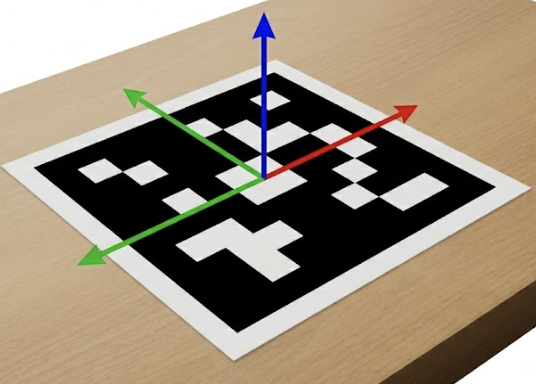
\includegraphics[width=0.6\textwidth]{Imagenes/Vectorial/codigoAruco.png}
    \caption{Ejemplo de marcador ArUco del diccionario 4$\times$4. El patrón binario interior
    codifica el identificador del marcador; el borde negro exterior facilita la detección del
    contorno.}
    \label{fig:codigoAruco}
\end{figure}


\subsection{Archivo de calibración}
\label{subsec:config_calibracion}

El plugin requiere los parámetros intrínsecos de la cámara que captura la escena para que la
estimación de pose sea métricamente correcta, tal como se describió en la
sección~\ref{subsec:pose_calibracion}. Estos parámetros se cargan desde un archivo generado
previamente con la herramienta de calibración incluida en el proyecto. El panel de propiedades
expone un selector de ruta que permite apuntar al fichero correspondiente a la óptica en uso.
Si se cambia de objetivo o de cámara durante la retransmisión, basta con actualizar este campo
y el plugin aplica los nuevos parámetros en el siguiente fotograma sin reiniciar la escena.


\subsection{Modelo 3D y textura}
\label{subsec:config_modelo}

El modo de modelo 3D estándar requiere especificar dos activos mediante selectores de fichero:

\begin{itemize}
    \item \textbf{Ruta del modelo 3D:} Ruta al fichero de geometría que se superpone sobre el
    marcador. El plugin acepta los formatos OBJ, FBX, DAE y GLTF a través de la biblioteca
    ASSIMP, por lo que el operador puede usar cualquier modelo exportado desde herramientas
    habituales de modelado 3D sin conversión previa. Al cambiar la ruta en directo, el plugin
    libera la geometría anterior de la VRAM y carga la nueva sin interrumpir la emisión.
    \item \textbf{Ruta de la textura:} Ruta a la imagen que se mapea sobre la superficie del
    modelo. Se aceptan los formatos PNG, JPG, BMP y TGA. Si el modelo ya incorpora referencias
    a texturas en su propio formato, este campo permite sobreescribirlas o substituirlas por
    una textura alternativa sin modificar el fichero del modelo.
\end{itemize}

\begin{figure}[H]
  \centering
  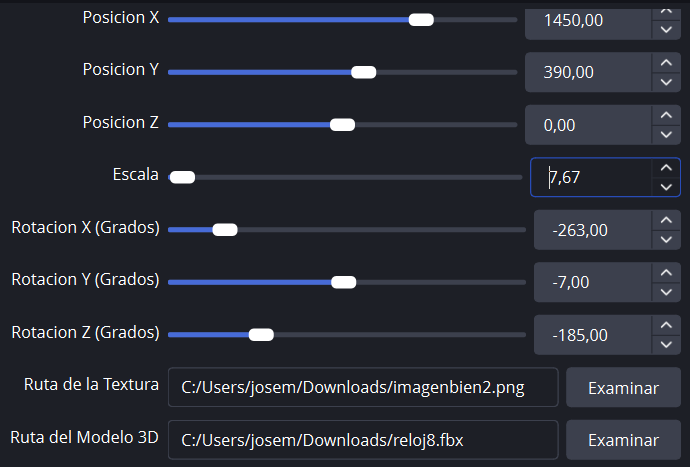
\includegraphics[width=0.72\textwidth]{Imagenes/Vectorial/UI_modo3D}
  \caption{Configuración del modo 3D en la interfaz del plugin: carga del modelo, textura, posición, rotación y escala.}
  \label{fig:ui_modo3d}
\end{figure}


\subsection{Offsets de posición, rotación y escala}
\label{subsec:config_offsets}

El panel expone dos familias de controles de ajuste fino (véase la sección~\ref{subsec:transformaciones_modelo} para los detalles matemáticos). La primera corresponde al \textbf{posicionamiento libre}, que permite situar el modelo directamente en coordenadas de pantalla mediante deslizadores de posición X, Y, Z y rotación (Pitch, Yaw, Roll) en grados; es útil para fijar una superposición en una esquina fija del encuadre independientemente de lo que la cámara capture. La segunda son los \textbf{offsets de modo AR}, que aplican una corrección relativa a la pose detectada para centrar el modelo sobre el ArUco o compensar inclinaciones del marcador. La figura~\ref{fig:ui_modo3dar} muestra el panel de propiedades con estos controles.

\begin{figure}[H]
  \centering
  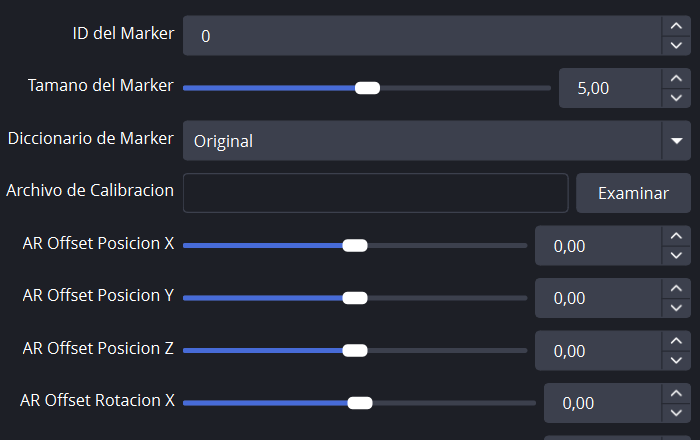
\includegraphics[width=0.72\textwidth]{Imagenes/Vectorial/UI_modo3DAR}
  \caption{Parámetros adicionales de la interfaz para el modo AR con modelo 3D: \textit{offsets} de posición y rotación relativos al marcador.}
  \label{fig:ui_modo3dar}
\end{figure}


\section{Conclusiones de la Descripción del Trabajo de Realidad Aumentada}
\label{sec:conclusiones_desarrollo_ra}

La fase de desarrollo técnico detallada en este capítulo ha permitido materializar los conceptos teóricos de visión por computador en una herramienta funcional e integrada dentro del ecosistema de OBS Studio. A través de la implementación del plugin, se han resuelto los desafíos críticos de latencia y precisión espacial que plantea la Realidad Aumentada en entornos de retransmisión en vivo.

El desarrollo ha validado que la arquitectura de \textit{filtro nativo} en OBS Studio es la solución óptima para este proyecto. Las principales metas alcanzadas en esta etapa incluyen:

\begin{itemize}
    \item \textbf{Eficiencia en la cadena de procesamiento}: La conversión de formatos de vídeo y la detección de marcadores ArUco se ejecutan directamente en el hilo de renderizado. Esto garantiza una sincronización total entre el mundo real y los elementos virtuales, evitando el desfase temporal.
    \item \textbf{Integración de Modelos 3D}: Se ha implementado un sistema de renderizado capaz de cargar y gestionar activos tridimensionales en la GPU. La gestión de buffers (VBO) y la vinculación dinámica de texturas permiten que los objetos aumentados se visualicen con coherencia visual y estabilidad sobre el entorno real.
    \item \textbf{Persistencia y Control}: El sistema permite al usuario ajustar parámetros críticos como \textit{offsets}, escalas y rotaciones de los modelos 3D en tiempo real. Estos ajustes se persisten automáticamente en la configuración del filtro de la escena, asegurando la versatilidad del sistema en futuras sesiones.
    \item \textbf{Gestión de Recursos}: Se ha diseñado un ciclo de vida estricto para el plugin que asegura la correcta liberación de la memoria RAM y VRAM (GPU), garantizando la estabilidad del software durante retransmisiones prolongadas.
\end{itemize}

Con la arquitectura de software finalizada y los módulos de detección y renderizado plenamente integrados, el sistema de Realidad Aumentada es capaz de situar y dibujar objetos 3D sobre un flujo de vídeo de forma precisa. Sin embargo, para que esta herramienta cumpla con los objetivos del proyecto, estos modelos 3D deben dejar de ser estáticos y comenzar a representar información dinámica y relevante.

Finalizada la descripción técnica del motor de RA, el siguiente capítulo, \textbf{Descripción del Trabajo para Concursos de Programación}~\ref{cap:descripcionTrabajoConcursosProgramacion}, se centrará en el desarrollo de la lógica necesaria para conectar este motor con fuentes de datos externas. En él se detallará cómo se consumen los datos de competición y cómo estos se transforman en las primitivas gráficas que el sistema de Realidad Aumentada acaba de definir.
